\documentclass[10pt, sigconf]{acmart}

\usepackage{booktabs} % For formal tables
\usepackage{multirow}
\usepackage[caption=false,font=normalsize,labelfont=sf,textfont=sf]{subfig}
% Copyright
%\setcopyright{none}
%\setcopyright{acmcopyright}
%\setcopyright{acmlicensed}
\setcopyright{rightsretained}
%\setcopyright{usgov}
%\setcopyright{usgovmixed}
%\setcopyright{cagov}
%\setcopyright{cagovmixed}


%% DOI
%\acmDOI{10.475/123_4}
%
%% ISBN
%\acmISBN{123-4567-24-567/08/06}
%
%%Conference
%\acmConference[SHORTNAME'17]{ACM Long Conference Name conference}{July 1997}{City, State, Country}
%\acmYear{2017}
%\copyrightyear{2017}
%
%\acmPrice{15.00}


\begin{document}
\title{NfvInsight: A Testbed for Benchmarking Network Function Virtualization}
%\titlenote{Produces the permission block, and copyright information}
%\subtitle{Extended Abstract}

\author{Tianni Xu$^{1,2}$    Sa Wang$^{1}$   Haifeng Sun$^{1,2}$   Xiufeng Sui$^{1}$   Xin Jin$^{3}$ Yungang Bao$^{1,2}$}
%\authornote{Note}
%\orcid{1234-5678-9012}
\affiliation{%
  \institution{1 State Key Laboratory of Computer Architecture, ICT, CAS}
  \streetaddress{2 University of Chinese Academy of Sciences}
  \city{3 Johns Hopkins University}
  %\state{State}
  %\postcode{Zipcode}
}
\email{{xutianni,wangsa,sunhaifeng,suixiufeng,baoyg}@ict.ac.cn, xinjin@cs.jhu.edu}


%\author{Sa Wang}
%%\orcid{1234-5678-9012} 
%\affiliation{%
%  \institution{Institute of Computing Technology, Chinese Academy of Science}
%}
%\email{wangsa@ict.ac.cn}
%
%\author{Haifeng Sun}
%%\orcid{1234-5678-9012}
%\affiliation{%
%  \institution{Institute of Computing Technology, Chinese Academy of Science}
%}
%\email{sunhaifeng@ict.ac.cn}
%
%\author{Xiufeng Sui}
%%\orcid{1234-5678-9012}
%\affiliation{%
%  \institution{Institute of Computing Technology, Chinese Academy of Science}
%}
%\email{suixiufeng@ict.ac.cn}
%
%\author{Xin Jin}
%%\orcid{1234-5678-9012}
%\affiliation{%
%  \institution{University of California, Berkeley}
%}
%\email{jxinpku@gmail.com}
%
%\author{Yungang Bao}
%%\orcid{1234-5678-9012}
%\affiliation{%
%  \institution{Institute of Computing Technology, Chinese Academy of Science}
%}
%\email{baoyg@ict.ac.cn}

% The default list of authors is too long for headers}
\renewcommand{\shortauthors}{F. Lastname et al.}


\begin{abstract}
Network function virtualization (NFV) has been gaining
more and more attention in both industry and academia.
Unfortunately, setting up an NFV environment is non-trivial.
By surveying authors of many SIGCOMM/SOSP/NSDI papers,
we learn that making NFV environments work actually is the most painful step
during these phd students' research and usually takes 1-2 human-month or even longer.
To facilitate NFV research, we introduce NfvInsight,
an NFV benchmark suite that features representative virtual network functions (VNFs),
one-click deployment and plenty metrics. Specifically,
NfvInsight provides a couple of representative VNFs and VNF-chains
and leverages Kubernetes and docker to ease VNF image packaging, virtualization management,
network configuration, generating network traffic and forwarding rule installation and so forth.
In this paper, we present a work-in-progress version of NfvInsight that
currently includes five VNFs %covering half of the NFV use cases,
and four typical VNF chains. Preliminary experiments demonstrate
that NfvInsight is able to meet the benchmarking requirements.
\end{abstract}

%
% The code below should be generated by the tool at
% http://dl.acm.org/ccs.cfm
% Please copy and paste the code instead of the example below.
%

%\begin{CCSXML}
%<ccs2012>
% <concept>
%  <concept_id>10010520.10010553.10010562</concept_id>
%  <concept_desc>Computer systems organization~Embedded systems</concept_desc>
%  <concept_significance>500</concept_significance>
% </concept>
% <concept>
%  <concept_id>10010520.10010575.10010755</concept_id>
%  <concept_desc>Computer systems organization~Redundancy</concept_desc>
%  <concept_significance>300</concept_significance>
% </concept>
% <concept>
%  <concept_id>10010520.10010553.10010554</concept_id>
%  <concept_desc>Computer systems organization~Robotics</concept_desc>
%  <concept_significance>100</concept_significance>
% </concept>
% <concept>
%  <concept_id>10003033.10003083.10003095</concept_id>
%  <concept_desc>Networks~Network reliability</concept_desc>
%  <concept_significance>100</concept_significance>
% </concept>
%</ccs2012>
%\end{CCSXML}
%
%\ccsdesc[500]{Computer systems organization~Embedded systems}
%\ccsdesc[300]{Computer systems organization~Redundancy}
%\ccsdesc{Computer systems organization~Robotics}
%\ccsdesc[100]{Networks~Network reliability}
%
%% We no longer use \terms command
%%\terms{Theory}
%
%\keywords{ACM proceedings}


\settopmatter{printacmref=false, printccs=false, printfolios=true}
\renewcommand\footnotetextcopyrightpermission[1]{}
\pagestyle{plain}
\maketitle


\section{Introduction}
Emerging network function virtualization (NFV) was initiated to replace hardware middleboxes with software implementation running in virtual machines (VMs), which would highly lower capital costs of network infrastructure and bring greater openness and flexibility.
% With the help of virtualization, we could manage multiple virtual network functions directly by standards virtualization management tools, as Openstack and K8s. could be directly managed by virtualization management tools, as Openstack, K8s.
% Virtualization bring much advantages to network functions, as ease of deployment, live migration, and so forth.
It is really exciting to encapsulate network functions into VMs, multiplexing underlying commodity, general purpose processors rather than dedicated physical boxes.
Thus NFV rapidly gained significant attentions by industry and academia. Plenty of works devote much effort to simplify building, deploying and managing NFs, like OpenNF \cite{gember-jacobson_opennf:_2014}, CoMb \cite{180672} and E2 \cite{palkar_e2:_2015}, or rewrite efficient NFs, like OpenBox \cite{bremler-barr_openbox:_2016} and Netbricks \cite{199352}.

% Network function virtualization (NFV) has become a hot topic, both in industry and academia.
% Since the publication of NFV Introductory White Paper \cite{} of ETSI in 2012, a lot of works have been emerged in this field. 
% Modification works of NFV were done on the whole software stack (or maybe both SW and HW stack?). 
% There are de facto industrial NFV platform OPNFV \cite{noauthor_home_nodate} as well as advanced NF allocation frameworks like OpenNF \cite{gember-jacobson_opennf:_2014}, CoMb \cite{180672} and E2 \cite{palkar_e2:_2015}. 
% Also, there are works like OpenBox \cite{bremler-barr_openbox:_2016} and Netbricks \cite{199352} to rewrite or modify the NFs.

%Embark\cite{194934}
%StateAlyzer\cite{194932}
%Split/Merge\cite{180307}
%ClickOS\cite{179771}
%APLOMB\cite{sherry_making_2012}
%FTMB\cite{sherry_rollback-recovery_2015}
%DFC\cite{194970}

However, although virtualization save much time of NFs management for us, building a NFV testbed still seems to be a time-consuming and annoying experience. We did a survey recently among experienced researchers on networking who claimed ever build a NFV testbed. Surprisingly, we find that it takes almost 1-2 months to build up a NF cluster with less than 10 VM instances. when the scale of instances increase to over 50, the buildup process extends to 3-4 months, or even more. One of our respondent said that they were still keeping on iterating and improving their testbed constantly. It is hard to imagine what a disaster it is for newcomers who intend to make some optimizations and contributions to the community. 

Therefore, we think that the time is ripe to consider a NFV benchmark suite that aims to greatly simplify the process of building a NFV testbed, especially for the newcomers. To fulfill this goal, we need to address three questions:
\textit{1) which are the representative NFs and NFs chains?} For the newcomers, it is frustrated to choose some representative NFs among NFs of various functions of various open source implementations. Besides, the order of NFs chained together is also important, and should be closed to the production environments as much as possible. Thus, the NFV benchmark should consist of a bunch of representative NFs and NFs chains widely accepted.
2) How to accelerate the buildup process? The most disturbing part of buildup process is to install and configure all the NFs one by one, with endless package dependency and manual reading. We should leverage the benefit of virtualization which is ``build once, run everywhere''.
3) what metrics should we collect and present? Last but not least, which metrics would be the proof of the measurement and demonstrate the effectiveness of the optimization?

Considering these questions, we present \textbf{NFVInsight}, a suite of NF benchmarks that help users set up their own NFV testbeds easily and rapidly. NFVInsight has following characteristics:
% However, even though a suite of easy-to-use NFV benchmark is not yet existed. It is unavoidable to experience a time consuming process finding both open source software and proper chaining policies. According to our observation, most NFs used in papers are different open source implementations linked in different kinds of NF chain policies. So that, there is not yet a general baseline for measurement and comparison. Furthermore, the workload generator and network traffic trace used are also different, traces need to be provided to test different NF chains.



% We also did a survey among top conference researchers who have experiences setting up NFV environment. In our survey, we found that the deploying time varies much due to the scale. In average, it takes 1-2 months to build up a NF cluster having less than 10 VM instances. But when the scale of instances increase to over 50, the build up process can take 3-4 months or more. One of our respondent said that they were still keeping on iterating and improving their testbed constantly.



% In this paper, we develop a suite of NF benchmarks, which is supposed to have the following characteristics: 1) Representing typical NFs 2) Easy to use 3) Plenty metrics for measurement.

% According to our research and observation,
% the representative of an NFV benchmark
% should be satisfied in three aspects:
%\begin{itemize}
%\begin{enumerate}
%\item{\textbf{Representative NFs.}}
\textbf{1) Representative NFs \& NF chains.}
we referred to the NFV Introductory White Paper \cite{},
which defined ten scenarios of NFV use cases.
In the first version of our benchmark,
the open source implementation of NFs we collected
covers half of the ten use cases.
Table \ref{nfs} lists the basic information of NFs used in our benchmark.
%\item{\textbf{Representative NF chains.}}
% \textbf{2) Representative NF chains.}
For NF chains, we referred to ETSI standard documents of SFC
(Service Function Chaining) \cite{draft-ietf-sfc-dc-use-cases-06}
for the typical use case of service chains
in the scenarios of both enterprise user and datacenter.
%We also consulted our industrial partners for real world chaining policies.
The typical NF chains our benchmark provides are listed in Table \ref{chains}.
%\item{\textbf{Proper workload generator.}}
\textbf{2) Proper workload generator.}
Since each NF chain serves at different network level,
only one workload generator is not enough to test all the scenarios.
So we select different clients for each chain.
%and fixed the content of each chain.
%\end{itemize}
%\end{enumerate}
\textbf{3) Easy to use.}
The goal of the `easy to use' design is to
achieve one-week setting up as well as one-click test running,
no matter the scale of the testing environment.
To finish a test, users only need to touch one configuration file
and execute one single command.
In the end, the measurement report will be output to a file.
To implement our design,
we leverage Docker and Kubernets to pack NFs in docker,
manage the images, and do allocation automatically.
We use OVS to do switching and packet force forwarding.
Pre-written scripts and Openflow rules are written
to implement chaining and flow control.
%There are more complains pointing out their pain points: 1) Automate the setting up and testing process. 2) Configure and stabilize NFs (?). 3) Write rules to set up topology and enforce flow control.
%%our design to solve the pain points????
%`easy to use' design should solve pain points
\textbf{4) Metrics.}
In our benchmark, we provide the most concerned metrics for measurement,
that is latency and throughput.
We measure latency in the granularity of per-packet and per-NF,
and output cumulative distribution of latency in the measurement report.

\textbf{Contributions.} We make the following contributions:



%The main contribution of our work is

%\section{Background and Motivation}
%
%\subsection{Network Function Virtualization}
%NFV involves multi-layers in the whole software stack,
%
%The concept of NFV chain

\section{A Survey of NFV Testing Environment Deploying}
%To further prove our observation,
To get first-hand information about researchers' experience on
the deployment of NFV testing environment,
we did a survey among top conference authors
dedicated in the field of NFV.
We delivered the survey to sixteen researchers
who are the first authors of their papers published on %published on top conferences
SIGCOMM/SOSP/NSDI of recent years
and we finally collected eight responses.

In the first place, we asked the number of types of VNF they used,
and the source of VNF, chaining policy and workload generator.
Averagely, six types of VNF are used in one paper.
Most of the VNF are open source implementations,
though three of our respondents have written their own VNF.
%a list of open source NFs found in papers??
The chaining policies are all found in papers or public policies.
And for workload generator,
half of researchers directly used open source software,
and half of them wrote by themselves.
%need some conclusion?

Another question we concerned most is
the time they spent on deploying a NFV testing environment.
To more precisely measure the labor time,
we use the metric of man-month
which indicates the number of months used
if the work is done by one person.
We also asked the scale of physical servers and VM instances,
as well as the virtualization technology they used.
The result is shown in Table \ref{survey}.

\begin{table}[!t]
\newcommand{\tabincell}[2]{\begin{tabular}{@{}#1@{}}#2\end{tabular}}
\centering
\begin{tabular}{|c|c|c|c|c|}\hline
& \tabincell{c}{Man-Month\\Used} & \tabincell{c}{\# of\\Servers} & \tabincell{c}{\# of\\VMs} & \tabincell{c}{Virtualization\\Technology}\\\hline
1 & $<$0.5 & 4 & 11-20 & KVM\\\hline
2 & 0.5-1 & 2 & 1-5 & Hyper-V\\\hline
3 & 0.5-1 & 4 & 1-7 & Container\\\hline
4 & 0.5-1 & 4 & 6-10 & KVM\\\hline
5 & 1-2 & 4 & 6-10 & \tabincell{c}{Container,\\KVM and other}\\\hline
6 & 4 & 10 & 100 & KVM\\\hline
7 & 3 & 24 & 72 & KVM\\\hline
8 & \tabincell{c}{Constantly\\Iterating} & 4 & 1-5 & Xen\\\hline
\end{tabular}
\caption{The result of our survey reflects the relationship
between labor consuming and the scale of the testing environment.}
\label{survey}
\end{table}

According to the feedback, we can see the average time
of deploying a testing environment for NFV is around 1-2 months
for a cluster that is not in very large scale.
It can be quite fast for a experienced person,
as the feedback No.1, who used less than half a month
setting up a cluster including 4 physical servers and 11-20 VMs.
However, for the others, the deploying process
can be time-consuming and painful.
Take feedback No.6 and No.7 as examples,
they built their test environment in quite large scale,
resulting in much longer setting up time.

setting up an NFV environment involves multi-layers in the whole software stack,
which includes virtualization, cluster management,
network virtualization, and NF configuration,
so that any point can become a bottleneck,
especially for a green hand.
Take respondent No.8 as an example,
Most problems they encountered are related to the hypervisor they used.
And respondent No.7 said they changed from Xen
to KVM with Openstack and things got much better.
We asked the authors for their most painful experiences,
and we summarize the reasons making the setting up time so long
as the following:

\begin{itemize}
\item[-]{}
Automating the process of setting up the testbed.
\item[-]{}
Setting up the datapath (interfaces, DPDK, routing tables, etc).
\item[-]{}
Installing proper rules in OpenFlow-enabled switches to enforce chaining.
\item[-]{}
Figure out appropriate workload to test different types of VNFs.
\item[-]{}
Figuring out how to determine that NFs were done starting up and ready to forward packets.
\end{itemize}

%Automating the process of setting up the testbed end to end took us a lot of time and many iterations.
%%No.4
%
%We wrote a bunch of scripts that simplified most of the process. The primary trouble was in figuring out how to determine that NFs were done starting up and ready to forward packets.
%
%Two parts for me:
%1. Install, configure and stabilize the open-source software, especially under heavy workload.
%2. Figure out appropriate workload to test different types of VNFs. It would be great if there is some real-world traffic/workload traces.
%
%Traffic generation and topology configuration
%
%Setting up the datapath (interfaces, DPDK, routing tables, etc)
%Installing proper rules in OpenFlow-enabled switches to enforce chaining

One of feedback pointed out that:

%\begin{itemize}
%\item[]{}
``If there is a system that will take as input key parameters (e.g., number of nodes, topology, VM images, choice of hypervisor) and then automatically generates a ready to go set up, that will be of a huge value!"
%!!!!but actually, we cannot...
%\end{itemize}

%This suggestion firms our intention to publish
The survey indicates the strong demand of an NFV benchmark
which provides typical NF services and workload generator,
automatically runs tests according to user configurations,
and reports the measurement results in the end.
In particular, the benchmark should support swift deployment
especially for large NF scale.



\section{Benchmark Description}

%\subsection{Overview}
According to our research and survey,
%we found that a suite of easy-to-use NFV benchmark is indeed.
the most urgent demand of an NFV benchmark is
to reduce the deployment time which includes
setting up virtualization platform and its network environment,
packing and managing VNF images,
writing scripts to automatically start NFs and chain them up.
Another requirement of the benchmark is to provide
representative VNF with widely accepted chaining policies,
as well as proper workload generator to drive the chains.
A suite of off-the-shelf benchmark can also
reduce the time spent on NF selecting.

In this paper, we introduce NfvInsight, an NFV testbed that meets these
requirements.
In this section, we first describe the overall architect of NfvInsight
and an brief instructions for a user to do deployment and testing.
Then we introduce the current NFs and chains of NfvInsight as well as
potential use cases.

%So, a selected suite of representative VNF
%with widely accepted chaining policy
%and proper workload generator is needed.
%%The idea of our work is based on an observation that
%Second, a well-designed benchmark with a bunch of
%pre-written scripts to automate the deployment process can effectively save time.
%Since NFV involves multi-layers in the whole software stack,
%the automation process includes VNF image packaging,
%NF allocation, networking config, forwarding rules installation,
%connection testing, and metrics measurement.
%%The goal and challenges of the work
%
%The goal of our work is to provide a benchmark suite
%with the following three characteristics:
%1) Representing typical NFs 2) Easy to use 3) Plenty metrics for measurement.

%Challenges:
%
%Representative NF
%
%K8s+ovs
%
%measurement

\subsection{Overview}

\begin{figure}[!t]
\centering
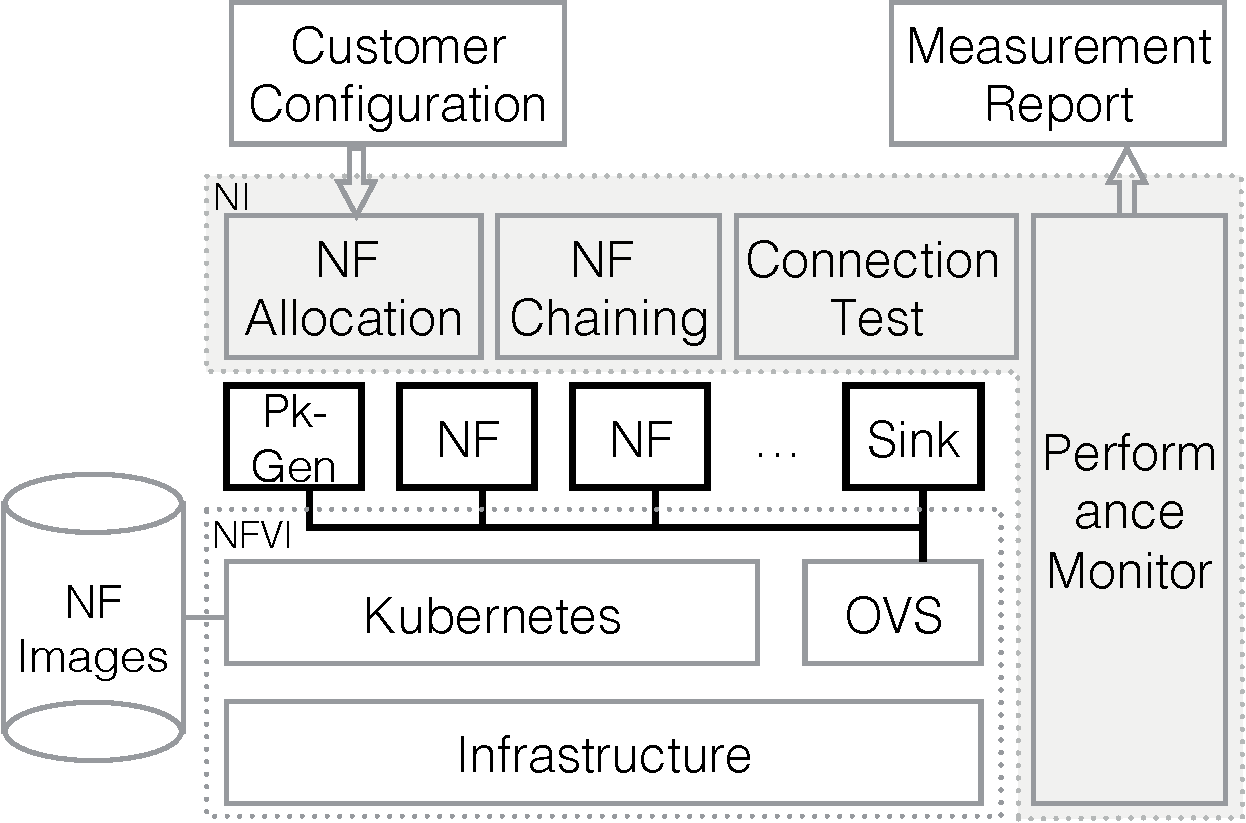
\includegraphics[width=3.3in]{fig/design2.pdf}
\caption{An overview of our benchmark design.}
\label{design}
\end{figure}

\begin{figure}[!t]
\centering
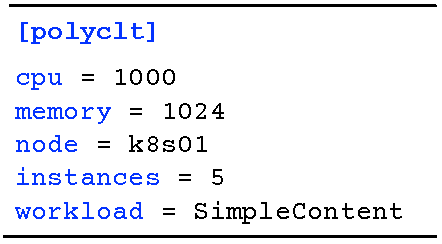
\includegraphics[width=1.8in]{fig/config_file.pdf}
\caption{An example of the config file format.}
\label{config}
\end{figure}

The overall architecture of NfvInsight benchmark is shown in Figure \ref{design}.
It has three main parts, NFVI, NF services and NI (the core of NfvInsight).
NFVI (NFV Infrastructure) consists of hardware resources
including compute, storage and network.
NF services are deployed upon NFVI, forming a service chain.
To leverage docker's light-weight isolation
and convenience of packing a runtime environment,
we chose to use Kubernetes as the infrastructure management framework,
which manages the physical cluster as well as the dockers and images.
OVS is used as the data path,
forwarding rules installed on OVS chains up the NF services.
The details of our network settings will be introduced in section 4.1.

NI (NfvInsight) is the key component of our benchmark
(highlighted in grey in Figure  \ref{design}),
which consists of a bunch of scripts
to automate the process of NF chain deployment.
To simplify its usage,
users are supposed to run only one command to start the test,
and touch only two files,
one configuration file and one measurement report.
NI reads in the customer configuration file (shown in Figure \ref{config}),
parse the file, and generate scripts to start docker, config network, and run NF.
%It does NF allocation and chaining automatically leveraging NFVI management framework.
Furthermore, the NI component is responsible for connection testing and performance monitoring
before regular tests.

The process for a researcher to use the benchmark includes five steps:

\begin{itemize}
\item[\textbf{1.}]{}\textbf{Run a pre-installed script.}
In our benchmark, a pre-installed script is provided to
help users install the prerequisite frameworks including Kubernetes and OVS
and complete configuration automatically.
%In the first step, users need to install Kubernetes, OVS
%and Openflow controller for their physical server cluster.
%Kubernetes is an open-source system for automating deployment, scaling,
%and management of containerized applications.
%To force forwarding packets cross nodes,
%OVS bridge and Openflow global control is needed.

\item[\textbf{2.}]{}\textbf{Download NF images or run an image-building script to build your owns.}
NfvInsight already provides several docker images. Alternatively, users can run a script to build
his own image locally. The image-building script helps build images listed in Table \ref{nfs} from DOCKERFILE, and setup a private image registry for docker creation in distributed cluster.

\item[\textbf{3.}]{}\textbf{Modify a configuration file.}
This configuration file is the only file needs user to edit.
NfvInsight provides a config template for each chain
designed in a uniform concise format shown in Figure \ref{config}.
The configurable variable includes resource of each docker,
mapping between physical server and docker,
number of NF instances, and other NF specific configurations.

\item[\textbf{4.}]{}\textbf{Run test with one command.}
Users can run the test by executing only one command.
NI does a series automate processes.
The details will be introduced in section 4.2.

\item[\textbf{5.}]{}\textbf{Get the report.}
The Performance Monitor module does metric measurement
and outputs a report.

\end{itemize}


\subsection{VNF}

\begin{table}[!htbp]
\newcommand{\tabincell}[2]{\begin{tabular}{@{}#1@{}}#2\end{tabular}}
\centering
\begin{tabular}{|c|c|c|}\hline
\textbf{Category} & \textbf{NF} & \tabincell{c}{\textbf{Workload}\\\textbf{Generator}}\\\hline
IMS & Clearwater & SIPps \\\hline
IDS & Snort & \multirow{2}{*}{Httperf} \\\cline{1-2}
NAT & iptables & \\\cline{1-2}
L4 Load Balancer & Haproxy & \multirow{2}{*}{Polygraph} \\\cline{1-2}
L7 Cache & Squid & \\\hline
\end{tabular}
\caption{NFs included in our benchmark.}
\label{nfs}
\end{table}

To select representative VNF,
%Since VNFaaS (VNF as a Service) and IMS are
%the most prevalent NFV use cases,
%we choose to .
We reviewed papers on NFV and found that they mainly use
open source implementations.
We grouped them into several categories according to their functionalities,
and selected those VNFs which need no modification to OS kernel.
NfvInsight provides DOCKERFILE to packet those VNFs into docker images,
and provides pre-defined config files to
config each VNF working in the way as demanded.
Table \ref{nfs} lists information of the VNFs
and the workload generators used.
Because iptables, Haproxy and Squid need real tcp requests,
packet trace replay cannot make them work properly,
we use Httperf to generate requests
and Apache Server to respond the requests.
Below are the brief introduction of the VNFs:

\begin{itemize}
\item{}
Clearwater \cite{noauthor_project_nodate} is an open source implementation of IMS (the IP Multimedia Subsystem) designed from the ground up for massively scalable deployment in the Cloud to provide voice, video and messaging services to millions of users.

\item{}
Snort \cite{snort} is an open source intrusion prevention system
capable of real-time traffic analysis and packet logging.
We config it working under intrusion detection model.

\item{}
Iptables \cite{Iptables}
We set particular rule to use iptables as DNAT and SNAT.

\item{}
Haproxy \cite{HAProxy} is a reliable, high performance TCP or HTTP load balancer.
We config it working under TCP mode to do L4 load balancing.

\item{}
Squid \cite{Squid} is a caching proxy for the Web supporting HTTP, HTTPS, FTP, and more. It reduces bandwidth and improves response times by caching and reusing frequently-requested web pages.
\end{itemize}

In current version of NfvInsight, we provide the following three workload generators.
SipP is specific for Clearwater,
while Httperf and Polygraph are used to drive the other service chains.
\begin{itemize}
\item{}
SIPp \cite{SIPp}
is a free Open Source test tool / traffic generator for the SIP protocol.
\item{}
Httperf \cite{Httperf}
is a tool for measuring web server performance. It provides a flexible facility for generating various HTTP workloads and for measuring server performance.
\item{}
Web Polygraph \cite{web-polygraph}
is a freely available performance testing tool for caching proxies, origin server accelerators, L4/7 switches, content filters, and other Web intermediaries.
\end{itemize}

\subsection{VNF Chain}

\begin{table*}[!htbp]
\newcommand{\tabincell}[2]{\begin{tabular}{@{}#1@{}}#2\end{tabular}}
\centering
\begin{tabular}{|l|l|l|}\hline
\textbf{} & \multicolumn{1}{c|}{\textbf{Sample Service Function Chains}} & \multicolumn{1}{c|}{\textbf{Chains in NI}} \\\hline
SFC1 & EdgeFW & Httperf/Polyclt $\to$ iptables $\to$ Apache/Polysvr \\\hline
SFC2 & EdgeFW $\to$ ADC & Httperf/Polyclt $\to$ iptables $\to$ Haproxy $\to$ Apache/Polysvr \\\hline
SFC3 & EdgeFW $\to$ ADC $\to$ AppFW & Polyclt $\to$ iptables $\to$ Haproxy $\to$ Snort $\to$ Polysvr \\\hline
SFC4 & WOC $\to$ EdgeFW $\to$ ADC $\to$ AppFW & Polyclt $\to$  Squid $\to$ iptables $\to$ Haproxy $\to$ Snort $\to$ Polysvr \\\hline
\end{tabular}
\caption{Sample VNF service function chains and chains provided by our benchmark.}
\label{chains}
\end{table*}

To find representative NF chaining policies,
we referred to IETF Service Function Chaining Use Cases
In Data Centers \cite{draft-ietf-sfc-dc-use-cases-06}.
The standard provides several sample service chains,
as listed in Table \ref{chains}, the second column.
The sample chains are connected by four network function concepts.
Definitions of each function concepts are given in the standard file,
and are listed in the following part of the paper.
The definitions are generalized,
actual implementations may vary and have functions overlapped.
We form the chains in our benchmark using the open sources
implementations in Table \ref{nfs} according to the sample chains.
The chains in NI are listed in Table \ref{chains}, the right column.

\begin{itemize}
\item
Edge Firewall (EdgeFW): Service functions such as VPN, DHCP, NAT, IP-Audit, Protocol Inspection, DPI etc., with policies primarily focusing on threats external to the data center.

\item
Application Delivery Controller (ADC): Service Function that distributes traffic across a pool of servers (applications) for efficient resource utilization, application scaling as well as to provide high availability among others.

\item
Application Firewall (AppFW): Service Function that isolates traffic within a segment or protects from application specific threats. This falls into the same class as DPI but deployed much closer to the applications. It is an intra-segment firewall.

\item
Web Optimization Control (WOC): Service functions to optimize the use of WAN link bandwidth, improve effective user throughput and latencies leading to overall improved user experience. WOC includes various optimizers such as compression, de-duplication, congestion control, application specific optimizers, etc. %WOC requires peers at either end of the WAN link to perform optimizations. The scope of this document is limited to the DC side of the WAN link.
\end{itemize}

% \begin{figure}[t]
% \label{cdf}
% \centering
% \includegraphics[width=3.3in]{cdf_chain1.pdf}
% \caption{Per-packet latency}
% \end{figure}

% \begin{figure}[t]
% \label{cdf}
% \centering
% 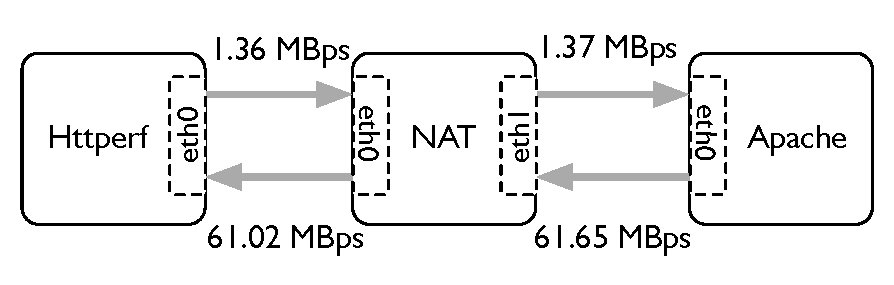
\includegraphics[width=3.3in]{throughput_chain1.eps}
% \caption{Throughput}
% \end{figure}

% \begin{figure}[t]
% \label{cdf}
% \centering
% 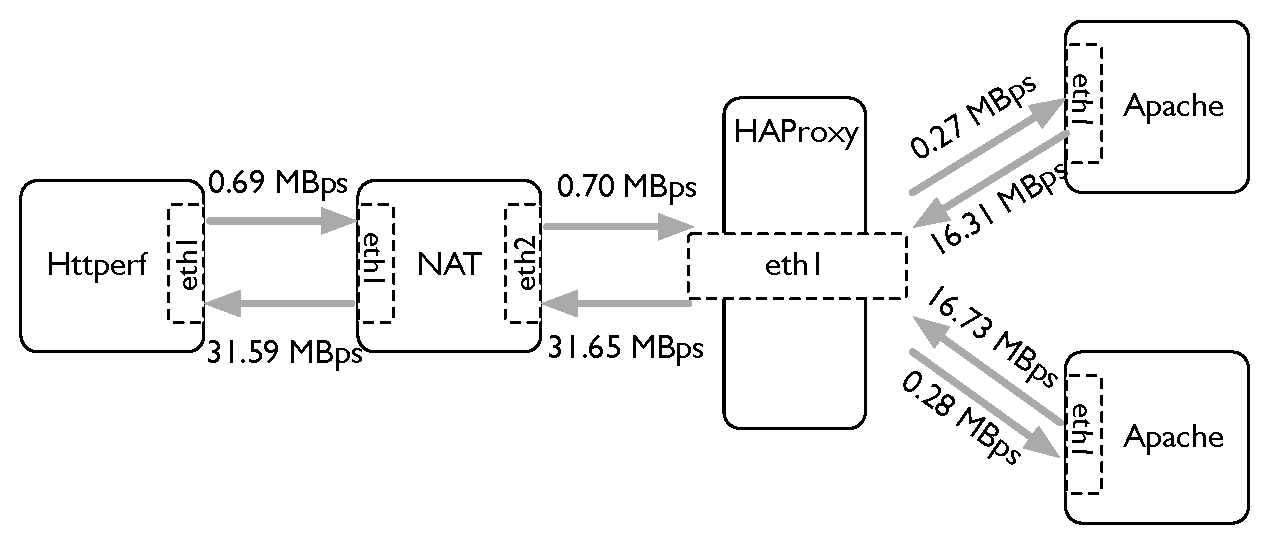
\includegraphics[width=3.3in]{throughput_chain2.eps}
% \caption{Throughput}
% \end{figure}


%\subsection{Use Case for NfvInsight}
%First, for all these researches, a universally used baseline is lacked
%for comparison experiments.

\section{Implementation}
NI is the core component of our benchmark,
it automates the process of running an NFV experiment.
In this section, we will introduce the multiple server network environment
which NI operates on,
as well as detailed implementation of NI.

\subsection{Multiple Server Network}

\begin{figure}[!t]
\centering
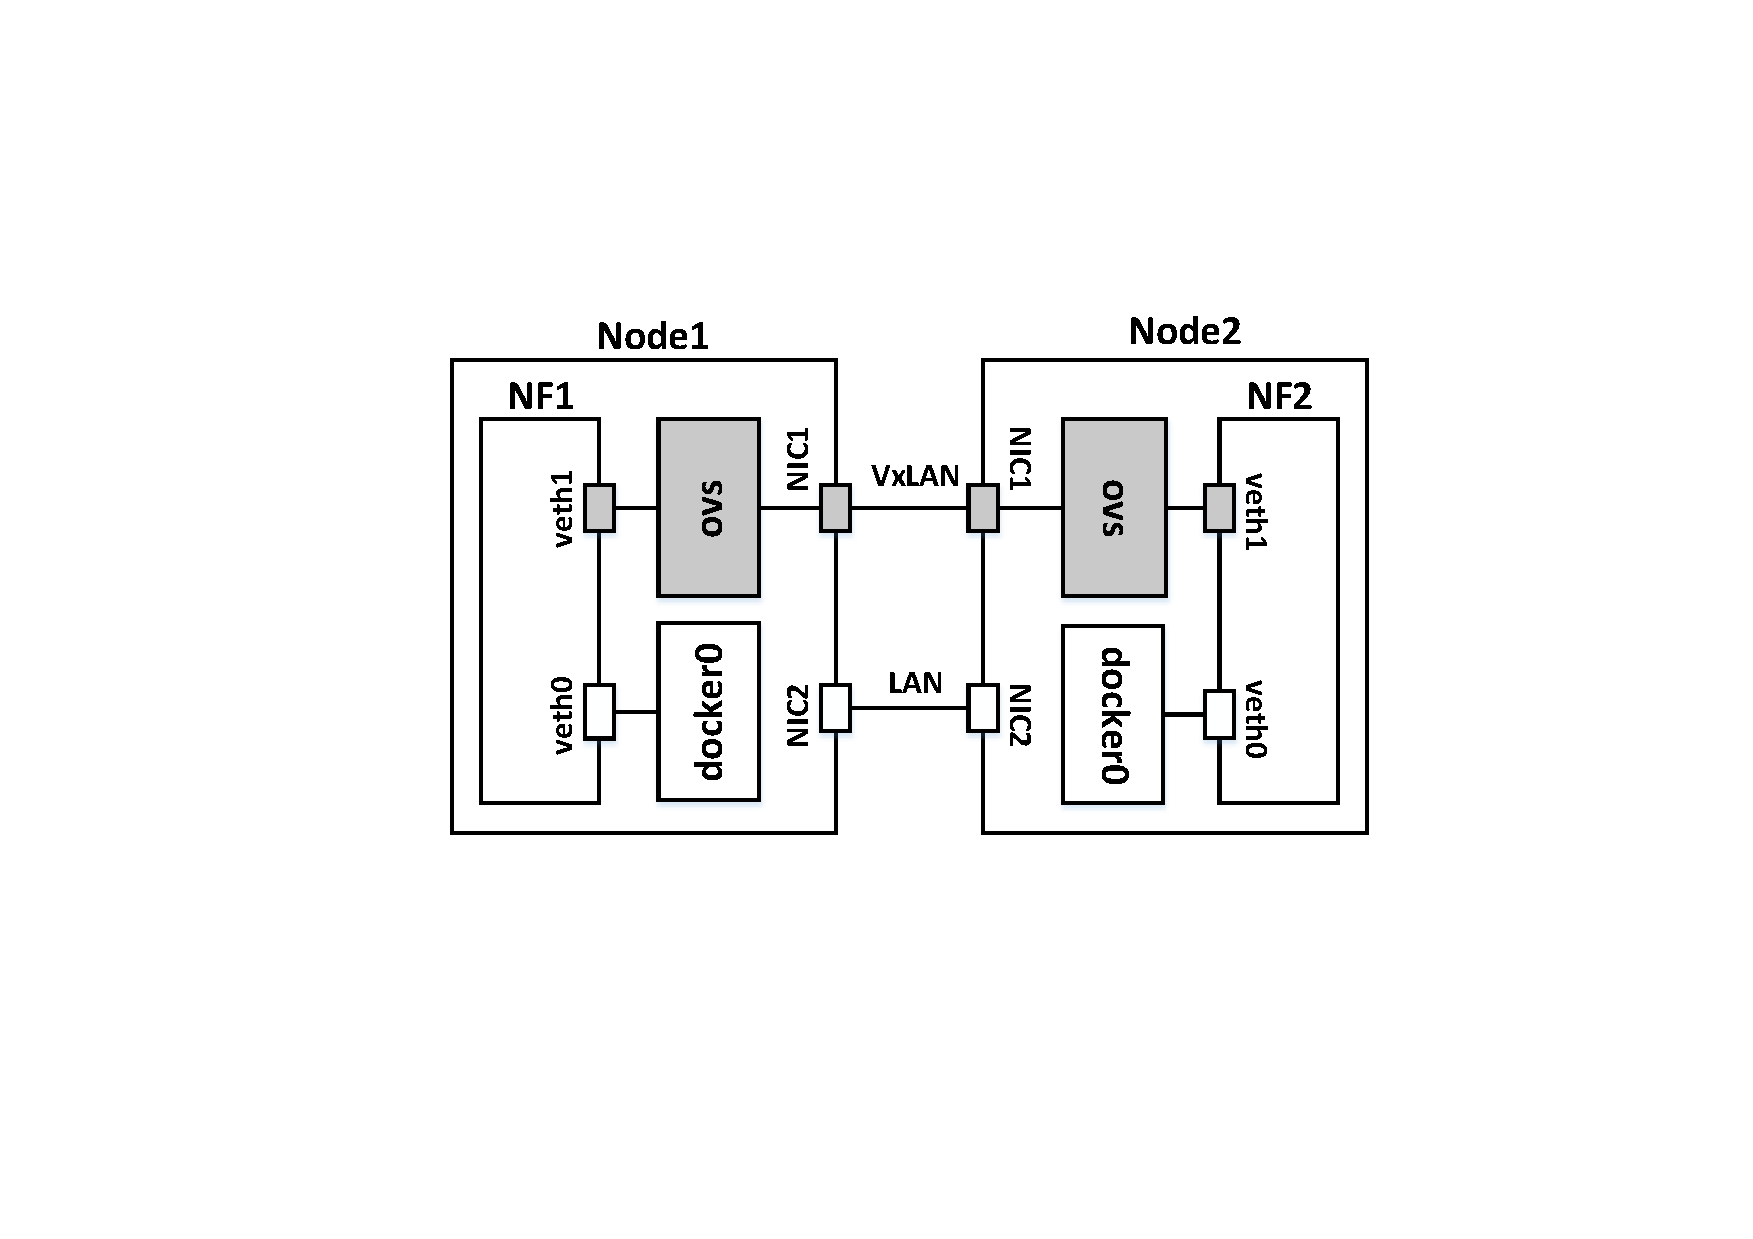
\includegraphics[width=2.7in]{fig/network.pdf}
\caption{Network of multiple server.}
\label{network}
\end{figure}

The network environment NI works on is shown in Figure \ref{network}. 
To setup a multiple server test environment, 
a LAN connection between servers is prerequisite. 
After Kubernetes installation, a Linux bridge named docker0 is setup 
to guarantee Kubernetes management and communication between dockers.
Because NFs needs forwarding control of flows, 
OVS and Openflow rules are needed. 
We setup OVS bridges and VxLAN connection in the pre-install script.
To setup data path for VNF, NI creates virtual net devices for dockers 
and  connect them to OVS bridge. 
The route marked in grey in Figure \ref{network} indicates the 
date path between VNFs.

\subsection{Auto Deploy}
To implement auto deployment, 
NI reads the configuration file edited by users shown in Figure \ref{config} 
and generate four types of scripts,
which includes SFC starting and delete scripts, 
docker resource definition file, and config file for specific NF.
Then the NF Allocation module deploys containers according to user configuration.
When containers are started and their status turn to `ready',
NF Chaining module adds virtual NIC for each container,
connects them to OVS bridge,
and installs Openflow forwarding rules according to the chaining policy.
To check whether the chain works,
the Connection Test module send a TCP request
from the packet generator and check if it gets response from Apache server.
If the connection test is passed,
the test is run and metric measurement begins.

%\subsection{Measurement}






\section{Evaluation}
The development of NfvInsight is still in process.
Although we have done most of automatic tools, the number of
available VNF-chains is limited. In this section, we only
demonstrate several preliminary experiments to basic functionality
of the NfvInsight testbed. As shown in Figure \ref{network},
our experiments are conducted on two
physical servers with Intel Xeon E5V3-2658 2.2GHz,
12 cores, 32GB DRAM, 10Gbps NICs. The servers run
CentOS 7 system, with Kubernetes 1.4 and Open vSwitch 2.5.1.
We encapsulates VNFs with Docker 1.12.5 running Ubuntu 14.14.
We use NfvInsight to deploy VNF-chains on single server
as well as two servers and measure network metrics
such as throughput and latency.
In this section, we mainly evaluate the first two chains in Table \ref{chains}.




%\subsection{Throughput}

%\begin{figure}[t]
%\label{cdf}
%\centering
%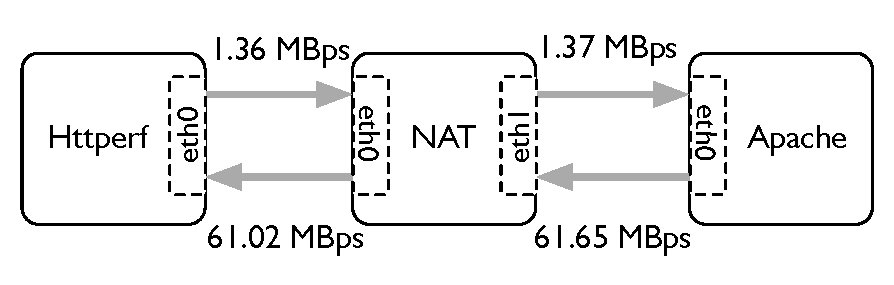
\includegraphics[width=3.3in]{throughput_chain1.eps}
%\caption{Throughput of each NF of SFC1.}
%\end{figure}
%
%\begin{figure}[t]
%\label{cdf}
%\centering
%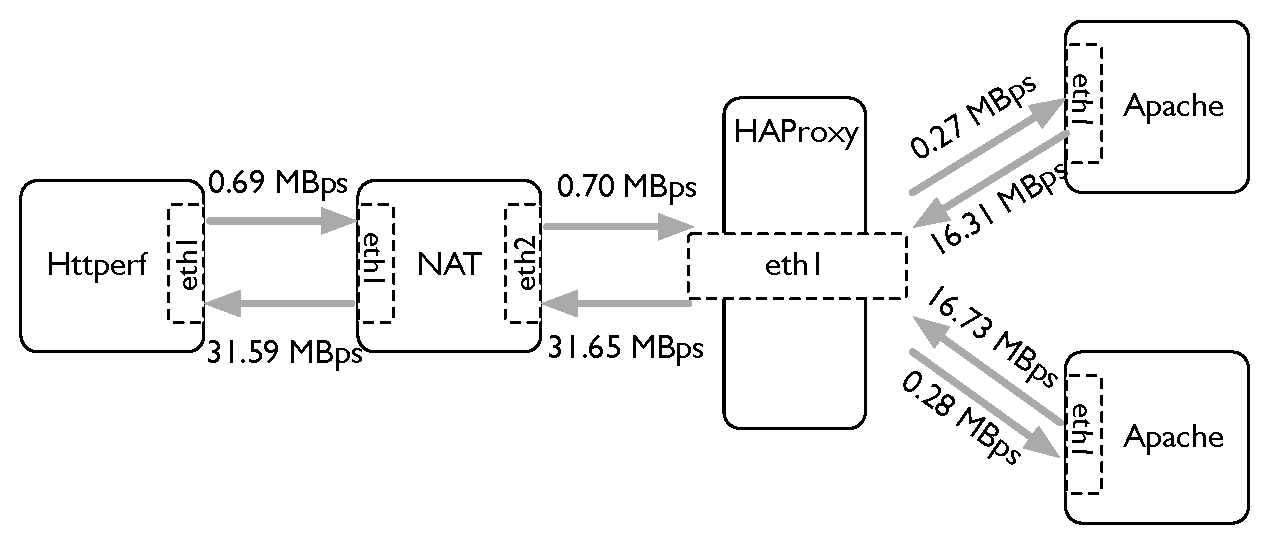
\includegraphics[width=3.3in]{throughput_chain2.eps}
%\caption{Throughput of each NF of SFC2.}
%\end{figure}

\begin{figure}[!t]
\centering
\subfloat[SFC1]{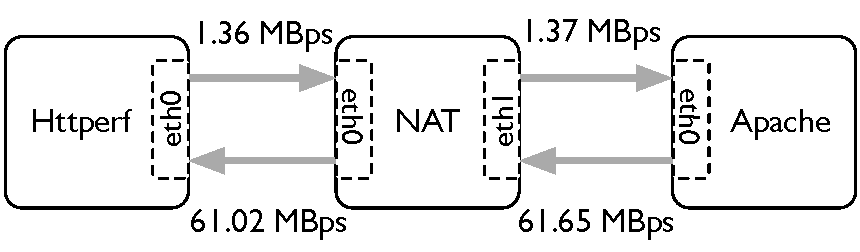
\includegraphics[width=3.3in]{fig/throughput_chain1.pdf}
\label{throughput_SFC1}}
\hfil
\subfloat[SFC2]{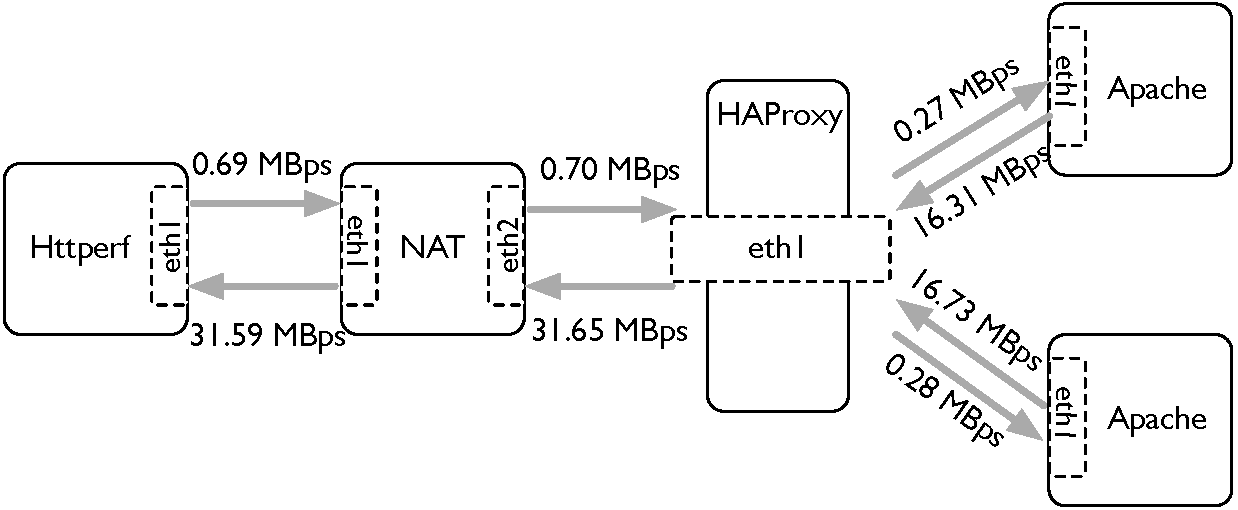
\includegraphics[width=3.3in]{fig/throughput_chain2.pdf}
\label{throughput_SFC2}}
\hfil
\caption{Throughput of each NF}
\label{throughput}
\end{figure}



% \begin{figure}[t]
% \centering
% 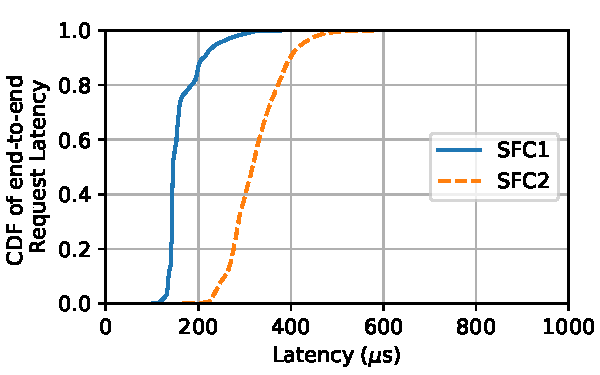
\includegraphics[width=3.3in]{fig/e2e_latency_chain12.pdf}
% \caption{End-to-end request latency of SFC1 and SFC2.}
% \label{e2e_latency}
% \end{figure}

We measure throughput of each VNF by using Docker API that
is able to record transmit bytes and receive bytes of each container. 
Throughput of each VNF is calculated
by doing subtraction of transmit bytes and dividing it by total testing time.
We also measure end-to-end latency of each request by modifying the workload generator Httperf,
which records the latency of each request and output the distribution of latencies.

Figure \ref{throughput} shows the topology of two chains
and the throughput are labeled on the arrows.
The direction of the arrows indicates the flow of the packets.
It is worth noting that 
we only need to modify 6 lines of configuration files
to form such two different VNF-chains. Once the configuration 
file is modified, we run only one command to deploy the two chains. 
This experiment demonstrate that NfvInsight is able to support 
fast configuration and deployment.


%\subsection{Latency}


% \begin{figure}[t]
% \centering
% \includegraphics[width=3.3in]{fig/cdf_chain1.pdf}
% \caption{Per-packet latency of NAT in SFC1}
% \label{nat_latency}
% \end{figure}

\begin{figure}
  \begin{minipage}[t]{0.47\columnwidth}
    \centering
    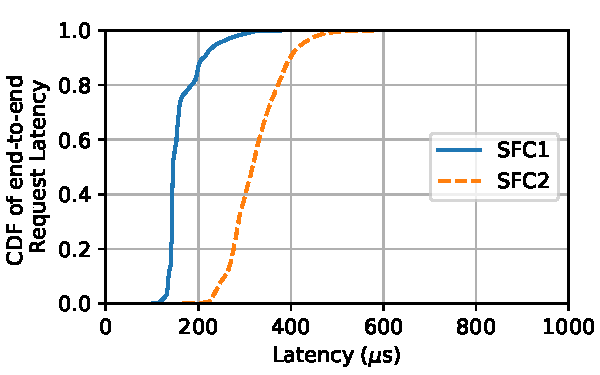
\includegraphics[width=4.0cm]{fig/e2e_latency_chain12.pdf}

    \caption{\small{End-to-end request latency of SFC1 and SFC2.}}
    \label{e2e_latency}
  \end{minipage}%
  \hfill
  \hfill
  \begin{minipage}[t]{0.47\columnwidth}
    \centering
    \includegraphics[width=4.0cm]{fig/cdf_chain1.pdf}
    \caption{\small{Per-packet latency of NAT in SFC1}}
    \label{nat_latency}
  \end{minipage}

\end{figure}

Figure \ref{e2e_latency} and Figure \ref{nat_latency} 
shows the end to end latency of SFC1 and SFC2 
as well as the per-packet latency of NAT in SFC1 respectively.
As mentioned before, to calculate per-packet latency, 
we slightly modified Httpperf to record latency of each request. 
For NAT's processing latency, NfvInsight leverages tcpdump to 
monitor and computer the latency of packets going through the NAT NFV. 
Currently, NfvInsight only provides two metrics, but we will add 
more metrics such as CPU utilization, memory working set size and cache miss rate.

The next experiments are conducted on two servers. Thank to 
Kerbuneters, NfvInsight can easily deploy VNFs on multiple servers. 
In our experiments, we use NfvInsight to deploy chain-1 and chain-2 
on two servers, as shown in Figure \ref{inter_throughput}. We can
see that the bandwidthes decrease compared to the deployment on
a single server. Then we modified 3 lines of the configuration file 
to increase the number of NAT and HAProxy instances, and deploy
the two chain again. By scaling out the two VNFs, the network 
bandwidths increase significantly, as shown in Figure \ref{inter_throughput}.
Thus, these experiments demonstrate that NfvInsight is able to 
perform the scale-out functionality, which is very important for NFV
deployment. 

\begin{figure}[!t]
\centering
\subfloat[SFC1]{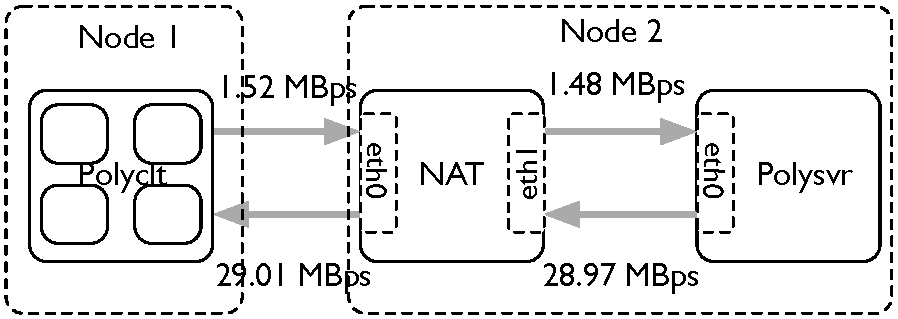
\includegraphics[width=2.9in]{fig/inter_node_chain1.pdf}
\label{inter_node_SFC1}}
\hfil
\subfloat[SFC2]{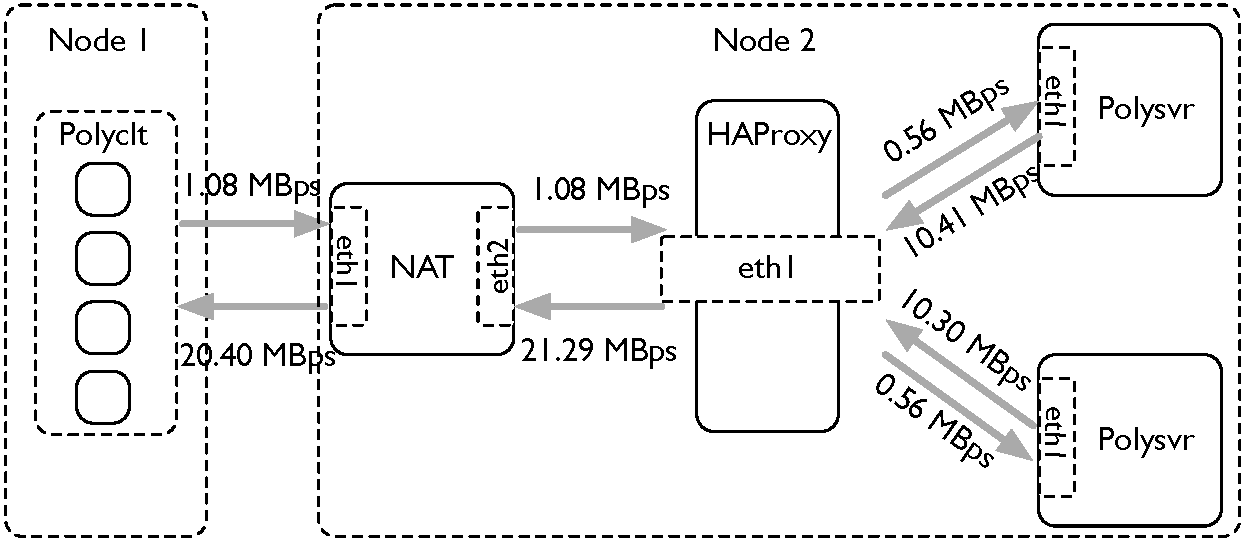
\includegraphics[width=2.9in]{fig/inter_node_chain2.pdf}
\label{inter_node_SFC2}}
\hfil
\caption{Throughput of each NF across two servers}
\label{inter_throughput}
\end{figure}


\begin{figure}[!t]
\centering
\subfloat[Before scale out]{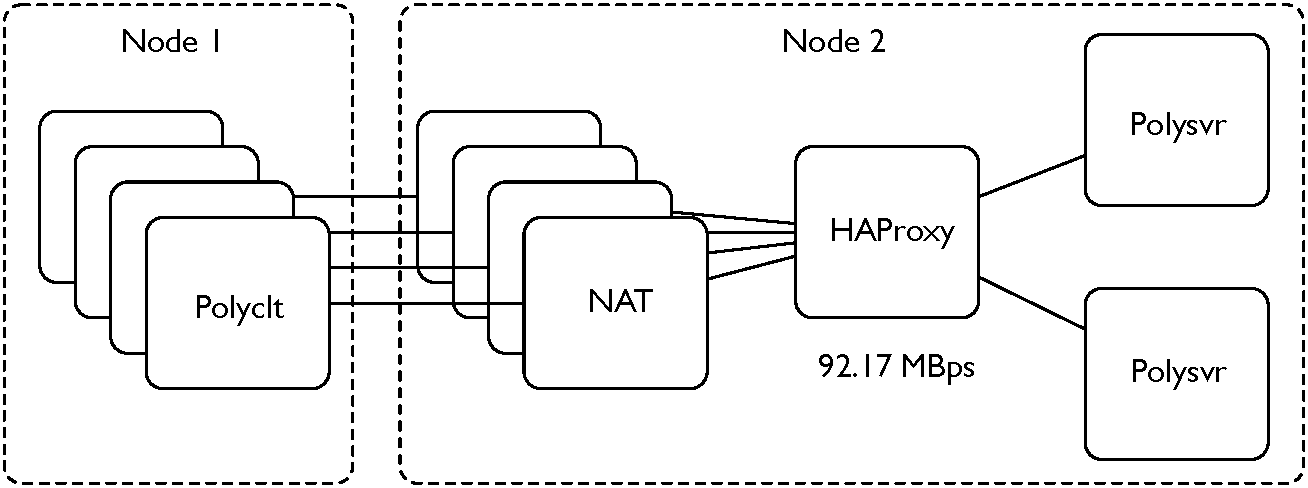
\includegraphics[width=3.3in]{fig/chain2extend1.pdf}
\label{1haproxy}}
\hfil
\subfloat[After scale out]{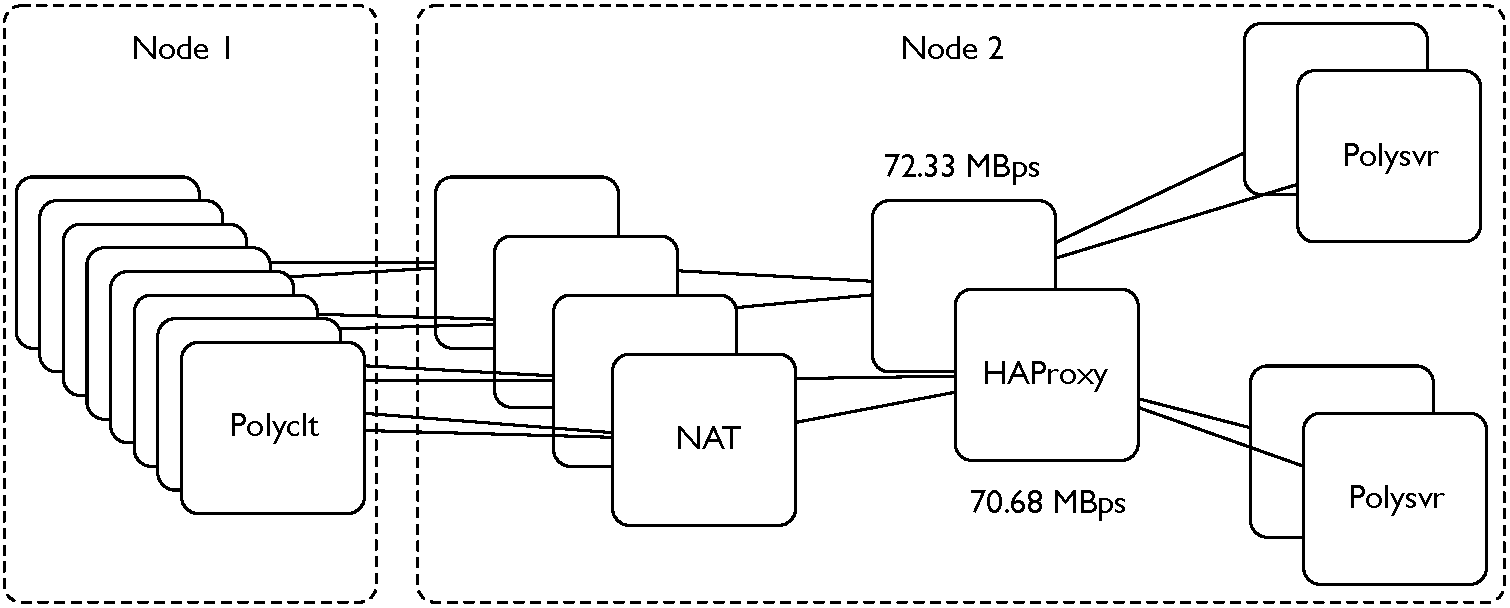
\includegraphics[width=3.3in]{fig/chain2extend2.pdf}
\label{2haproxy}}
\hfil
\caption{Throughput of SFC2 before and after HaProxy scaling-out.}
\label{scaleout_throughput}
\end{figure}


\section{Conclusions}

This paper is addressing how to ease NFV deployment for research,
which has been one of the most time-consuming and painful step according 
to our survey.We propose an NFV benchmark suite NfvInsight to offer
researchers a self-contained testbed. We carefully chose 
a couple of representative VNFs and VNF-chains and adopted 
Kubernetes and docker to ease deployment. This paper prepsents
a work-in-process version of NfvInsight that already have five VNFs
and four VNF-chains. Preliminary experiments demonstrated
that NfvInsight is able to fast deploy NFV environment on single physical
server or multiple servers. Our future work is to complete the 
rest functionalities of NfvInsight and make it open-source to the
NFV research community. 

\bibliographystyle{ACM-Reference-Format}
%\bibliographystyle{abbrv}
\bibliography{NFV_bib,NFV,sigproc}

%
%\bibliography{sigproc}

\end{document}
